\documentclass[cn]{elegantbook}
\usepackage[square,numbers,sort&compress]{natbib}
\newcommand{\upcite}[1]{\textsuperscript{\textsuperscript{\cite{#1}}}}
\usepackage{diagbox}
\usepackage{algorithm}
\usepackage{algorithmicx}
\usepackage{algpseudocode}
\renewcommand{\algorithmicrequire}{\textbf{输入:}}
\renewcommand{\algorithmicensure}{\textbf{输出:}}

\tikzstyle{startstop} = [rectangle, rounded corners, minimum width = 2cm, minimum height=1cm,text centered, draw = black, fill = red!40]
\tikzstyle{arrow} = [->,>=stealth]

% title info
\title{模式识别作业2}
\subtitle{在人脸数据库上应用PCA}
% bio info
\author{罗雁天}
\institute{清华大学电子系}
\version{2018310742}
\date{\today}
\logo{logo.png}
\cover{cover.jpg}

\begin{document}

\maketitle
\tableofcontents
\mainmatter
\hypersetup{pageanchor=true}
% add preface chapter here if needed
\chapter{问题描述}

本次作业为在人脸数据库上应用PCA。给定了face文件夹,其中有train和test两个文件夹。利用train中的人脸数据训练主成分分量,并完成以下练习。
\begin{enumerate}[(a)]
	\item 从train文件夹中随意取出一张图片向量$x$,将$x$投影到前$K$个主成分中,然后利用这些投影分量来重建人脸$x'$,并计算重建误差$||x'-x||^2$。从$K=1$开始,不断地增加$K$,给出重建误差随$K$的增长的收敛曲线。重建误差能否为0.
	\item 从test文件夹里读取文件名为“face.jpg”的文件,按照(a)的方式来做。与(a)相比,对于相同的误差阈值,是否需要更大的K?重建误差能否为0?
	\item 从test文件夹里读取文件名为“nonface.jpg”的文件,按照(a)的方式来做。与(b)相比,对于相同的误差阈值,是否需要更大的K?重建误差能否为0?
\end{enumerate}

\chapter{算法描述}
本次作业使用主成分分析算法(PCA)对图像进行主成分分析并且对图像进行重建,输入的训练集为500张$19\times 19$的人脸图像,首先使用PCA算法对训练集图像进行处理,得到人脸图像的主成分,然后将测试图像投影到主成分张成的空间,并用投影向量对原图像进行重建。主成分选取的特征维度不同,重建误差也不同,详细算法如Algorithm \ref{alg:pca}所示。

\begin{algorithm}[H]
	\caption{\label{alg:pca}使用PCA对人脸图像重建算法}
	\begin{algorithmic}[1]
		\Require 训练集图像(500张$19\times19$),测试图像($x$),主成分数量($K$)
		\Ensure 重建误差(error)
		\State 将$19\times 19$的训练图像拉平成$1\times 361$的向量,并且将500张图像向量组成$500\times 361$的矩阵$X$;
		\State 计算$X$的协方差矩阵$\Sigma = X^TX$
		\State 对$\Sigma$进行特征值分解;
		\State 将前$K$个最大特征值对应的特征向量组成投影矩阵$W$;
		\State 将测试图像($19\times 19$)拉平成$361\times1$的向量$x$,计算其均值为$\mu$;
		\State 计算投影$y=W^T(x-\mu)$;
		\State 计算重建向量$x'=Wy+\mu$;
		\State 计算重建误差$error=||x-x'||_2^2$;
	\end{algorithmic}
\end{algorithm}

\chapter{实验结果}
\section{实验结果}
\begin{figure}[!ht]
	\centering
	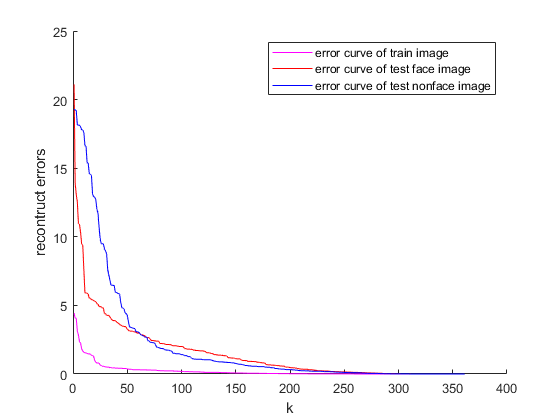
\includegraphics[width=\textwidth]{images/error}
	\caption{\label{fig1}图像重建误差与主成分数量$K$的收敛曲线}
\end{figure}

\begin{table}[!ht]
	\centering
	\caption{\label{tab1}不同误差阈值情况下三个图像所需要的K值}
	\begin{tabular}{|c|c|c|c|}
		\hline
		\diagbox{误差阈值}{所需K值}{图像} & train/face00018.jpg & test/face.jpg & test/nonface.jpg \\
		\hline
		5 & 1 & 24 & 45 \\
		\hline
		1 & 20 & 156 & 129 \\
		\hline
		0.1 & 142 & 267 & 258 \\
		\hline
		0.01 & 227 & 305 & 299 \\
		\hline
		0.001 & 286 & 320 & 323 \\
		\hline
		0.0001 & 317 & 357 & 355\\
		\hline
	\end{tabular}
\end{table}

\begin{table}[!ht]
	\centering
	\caption{\label{tab2}不同K值情况下三个图像的重建误差}
	\begin{tabular}{|c|c|c|c|}
		\hline
		\diagbox{K值}{重建误差}{图像} & train/face00018.jpg & test/face.jpg & test/nonface.jpg \\
		\hline
		10 & 1.58774 & 7.60218 & 17.61315 \\
		\hline
		61 & 0.30845 & 2.97574 & 3.03182 \\
		\hline
		62 & 0.30184 & 2.89951 & 2.88945 \\
		\hline
		360 & 1.35995$\times 10 ^{-8}$ & 6.02949$\times 10 ^{-5}$ & 2.55785$\times 10 ^{-5}$ \\
		\hline
		361 & 1.57945$\times 10 ^{-29}$ & 7.22276$\times 10 ^{-29}$ & 9.35632$\times 10 ^{-29}$ \\
		\hline
	\end{tabular}
\end{table}

我们选择训练集中的“face00018.jpg”,测试集中的“face.jpg”和“nonface.jpg”进行实验,将实验要求的3个问题统一绘制图像如图\ref{fig1}所示。为了更加清晰的讨论实验结果,我们将不同误差阈值情况下三个图像所需要的K值列表如表\ref{tab1}所示,并且选择了几个特殊的K值,列表展示了三个图像的重建误差如表\ref{tab2}所示.

为了直观的观察重建效果,我们选择了几个$K$值,将原始图像与重建图像列表如表\ref{tab3}所示
\begin{table}[!ht]
	\centering
	\caption{\label{tab3}不同K值情况下三个图像的重建图像}
	\begin{tabular}{|c|c|c|c|}
		\hline
		\diagbox{K值}{重建图像}{图像名} & train/face00018.jpg & test/face.jpg & test/nonface.jpg \\
		\hline
		原始图像 & 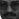
\includegraphics{../train/face00018}& 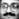
\includegraphics{../test/face}& 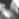
\includegraphics{../test/nonface} \\
		\hline 
		10 & 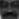
\includegraphics{../results/face00018_10}& 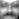
\includegraphics{../results/face_10}& 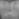
\includegraphics{../results/nonface_10} \\
		\hline 
		50 & 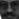
\includegraphics{../results/face00018_50}& 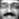
\includegraphics{../results/face_50}& 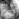
\includegraphics{../results/nonface_50} \\
		\hline 
		100 & 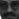
\includegraphics{../results/face00018_100}& 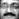
\includegraphics{../results/face_100}& 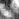
\includegraphics{../results/nonface_100} \\
		\hline 
		150 & 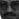
\includegraphics{../results/face00018_150}& 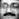
\includegraphics{../results/face_150}& 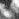
\includegraphics{../results/nonface_150} \\
		\hline 
		200 & 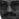
\includegraphics{../results/face00018_200}& 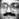
\includegraphics{../results/face_200}& 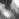
\includegraphics{../results/nonface_200} \\
		\hline 
		250 & 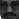
\includegraphics{../results/face00018_250}& 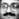
\includegraphics{../results/face_250}& 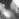
\includegraphics{../results/nonface_250} \\
		\hline 
		300 & 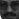
\includegraphics{../results/face00018_300}& 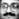
\includegraphics{../results/face_300}& 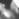
\includegraphics{../results/nonface_300} \\
		\hline 
		350 & 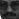
\includegraphics{../results/face00018_350}& 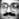
\includegraphics{../results/face_350}& 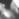
\includegraphics{../results/nonface_350} \\
		\hline 
		361 & 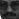
\includegraphics{../results/face00018_361}& 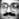
\includegraphics{../results/face_361}& 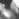
\includegraphics{../results/nonface_361} \\
		\hline
	\end{tabular}
\end{table}

从图中和表中我们可以看出:
\begin{itemize}
	\item 当$K=361$时,三个图像的重建误差分别为1.57945$\times 10 ^{-29}$、7.22276$\times 10 ^{-29}$和9.35632$\times 10 ^{-29}$,此时可以认为重建误差为0,这也非常容易理解,当$K=361$时,保留了特征空间的所有信息,图像可以没有损失的投影到特征空间,相当于一次正交变换,因此可以无损重建;
	\item 相同$K$值的情况下,训练集图片的重建误差最小,也就是说,在相同重建误差阈值的情况下,测试集的两张图片相比于训练集的图片需要更大的$K$值。
	\item 当$K\le 61$时,“face.jpg”的重建误差小于“nonface.jpg”,即在此种情况下,相同重建误差阈值时,“nonface.jpg”需要更大的$K$值,由此可见,特征空间很好的抓住了人脸特征;当$K\ge 62$时,“face.jpg”的重建误差大于“nonface.jpg”,即在此种情况下,相同重建误差阈值时,“face.jpg”需要更大的$K$值,此时是因为“nonface.jpg”图案较简单,因此在较多细节特征时,能够更好的重建;
\end{itemize}

\section{反思与总结}
观察训练集数据我们可以发现给出的人脸均为外国人的人脸,并且测试图片也是外国人脸数据,众所周知,中国人的人脸和外国人还是有差别的,因此对于中国人脸,使用此训练集训练pca进行重建的效果可能会有所不同,因此,在本小节,拿自己学生证的照片作为测试数据进行重建,与题目给出的外国人脸数据进行对比,得出实验结果。首先对我自己学生证上的照片进行裁剪,裁剪出人脸的区域,然后将其转换为灰度图并resize到$19\times19$,然后将此图像与训练集图片、测试集face图片进行对比,绘制出重建error曲线如图\ref{fig2}所示,从中可以发现,我自己的照片的重建误差居然奇迹般的和训练集数据的重建误差相近,比测试集的face图像的重建误差要小,难道是因为我自己照片裁剪出的区域看起来像外国人,interesting!

\begin{figure}[!ht]
	\centering
	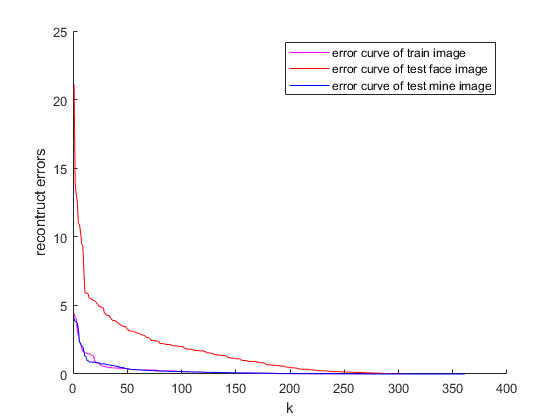
\includegraphics[width=\textwidth]{images/error2}
	\caption{\label{fig2}图像重建误差与主成分数量$K$的收敛曲线}
\end{figure}

看来由人脸数据训练pca进行重建对人脸的重建都有比较好的效果,因此我们在此选择了不是人脸的脸进行实验。在此,我们选择了《白蛇缘起》中小白的脸进行重建,众所周知,动漫中的脸和真实的脸差异还是挺大的,那么对于这次的重建效果会怎样呢,我们依然与训练集图片、测试集face图片进行对比,绘制出error曲线图如图\ref{fig3}所示。Exciting,可以看出动漫人物人脸的重建误差果然要比真实人脸的重建误差大,这也说明使用pca重建的话,针对不同的脸要训练不同的主成分来进行重建,对于动漫人脸,我们可以选择动漫人脸进行训练,然后再进行重建。

\begin{figure}[!ht]
	\centering
	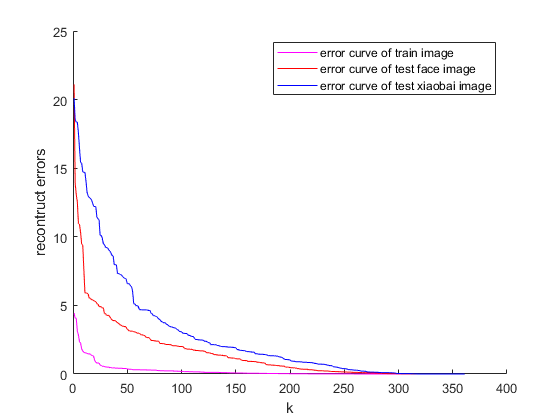
\includegraphics[width=\textwidth]{images/error3}
	\caption{\label{fig3}图像重建误差与主成分数量$K$的收敛曲线}
\end{figure}


\chapter{代码说明}
本次实验使用Matlab语言编写,所有代码放置在“code/”文件夹下:
\begin{itemize}
	\item main.m: 本次实验的主程序,直接执行便能得到图\ref{fig1}以及将重建之后的图像保存在“results/”文件下;
	\item read\_train\_images.m: 读取训练集图片,并将其构建一个$500\times 361$的矩阵;
	\item reconstruct.m: 重建图像的函数,输入训练数据$500\times 361$的矩阵,测试图像文件名和$K$值,输出重建误差以及重建之后的图像。
\end{itemize}


\end{document}